%\begin{frame}{titel}
%    \pause
%    \begin{columns}
%        \begin{column}{0.5\textwidth}
%            \begin{itemize}
%                \item <->
%                \item <->
%                \item <->
%                \item <->
%                \item <->
%                \item <->
%            \end{itemize}
%        \end{column}
%        \begin{column}{0.5\textwidth}
%            \centering
%            \only <->{
%                \includegraphics[scale=0.25]{images/}\\[-0.5\baselineskip]
%                \hspace{1.5cm}}%\href{www. ...}{[name, paper]}
%             }
%        \end{column}
%    \end{columns}
%\end{frame}
\section{Beschreibung des Probenkörpers}
\begin{frame}{Beschreibung des Probenkörpers}
    \pause
    \begin{columns}
        \begin{column}{0.5\textwidth}
            \begin{itemize}
                \item <1-> 3 Schichten plus Gitter
                \begin{itemize}
                    \item <2-> Substrat: GaAs (hier schwarz)
                    \bigskip
                    \item <3-> Pufferschicht: CdMgTe $\SI{4,6}{\micro\meter}$
                    \item <3-> Quantentopf: CdMnTe $\SI{10}{\nano\meter}$
                    \item <3-> Deckschicht: CdMgTe $\SI{30}{\nano\meter}$ 
                    \bigskip
                    \item <4-> Goldgitter mit einer Periode von $\SI{250}{\nano\meter}$
                \end{itemize}
                \bigskip
                \item <5-> CdMnTe ist ein semimagnetischen Halbleiter (DMS)
                \item <6-> Im QW entstehen Exzitonen
                \item <7-> zwischen Deckschicht und Goldgitter entstehen Plasmonen
            \end{itemize}
        \end{column}
        \begin{column}{0.5\textwidth}
            \centering        
            \only <1->{    
            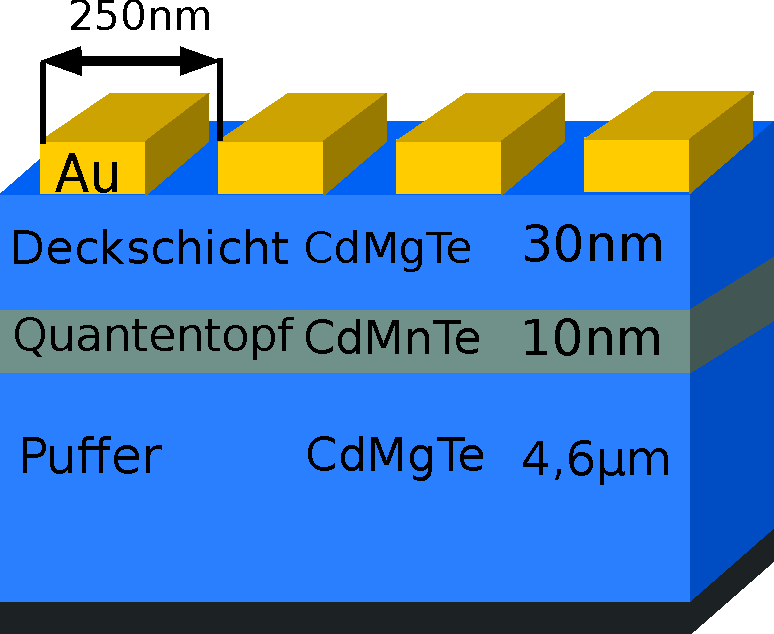
\includegraphics[scale=0.3]{images/probe.pdf}\\[-0.5\baselineskip]  }              
        \end{column}
    \end{columns}
\end{frame}